\chapter{Principi di Laser e Telemetria}
\label{capitolo1}
\thispagestyle{empty}

\textit{In questo Capitolo verranno richiamati i concetti fondamentali relativi al funzionamento delle sorgenti laser. Verranno quindi descritte le principali tipologie di sorgenti e le classi di sicurezza che ne regolamentano l'utilizzo. Successivamente, verr\'a esposto lo stato dell'arte dei misuratori ottici di distanza assoluta, ponendo particolare attenzione alle tecniche di misura a triangolazione, a tempo di volo e a onda continua. In conclusione, quest'ultime verranno messe a confronto con una tecnica alternativa, l'interferometria a retroiniezione, al fine di motivare l'utilizzo di tale tecnica per questo lavoro di Tesi.}

\section{Principi di funzionamento del laser}
LASER \'e l'acronimo di \emph{Light Amplification by Stimulated Emission of Radiation}, cio\'e luce amplificata dall'emissione stimolata di radiazione~\cite{sveltolaser}. In generale, un laser \'e un dispositivo elettronico in grado di emettere un fascio di luce.
%Un fascio di luce \'e un'onda elettromagnetica costituita da particelle chiamate fotoni. Il fotone \'e il quanto di energia della radiazione elettromagnetica.
La luce ha una natura duale; infatti si comporta sia come un'onda elettromagnetica che come una particella, detta fotone, che costituisce il quanto di energia della luce. 

Il fascio di luce emesso da un dispositivo laser possiede tre caratteristiche principali:
\begin{enumerate}
	\item Coerenza
	\item Monocromaticit\'a
	\item Direzionalit\'a
\end{enumerate}

Un onda \'e coerente spaziale se esiste una differenza di fase costante tra due punti qualunque sul fronte d'onda. Mentre, la coerenza temporale \'e strettamente legata al tempo di coerenza. Esso \'e l'intervallo medio di tempo nel quale l'onda compir\'a un certo numero di oscillazioni prima di cambiare fase.

La seconda propriet\'a garantisce che %(tutti i fotoni generati)
tutte le onde generate per effetto dell'emissione stimolata risultino iso-frequenziali, ovvero aventi tutti la stessa frequenza. Essa \'e strettamente correlata alla coerenza temporale.

La terza e ultima propriet\'a, invece, afferma che la radiazione emessa dalla sorgente si propaga nello spazio in un'unica direzione ben definita con piccoli angoli di divergenza del fascio parallelo e perpendicolare, pi\'u precisamente, l'angolo solido sotteso da un fascio laser \'e estremamente piccolo. Essa \'e strettamente correlata alla coerenza spaziale.


\subsection{Emissione stimolata di radiazione}
Il fenomeno che permette il funzionamento del laser \'e l'emissione stimolata, per questo \'e importante capire di cosa si tratta e in che modo essa \'e differente dall'emissione spontanea. Per fare ci\'o \'e conveniente richiamare alcuni concetti di base.

Come accennato in precedenza, la propagazione della luce nello spazio si sviluppa tramite particelle dette fotoni (o quanti), aventi ciascuna una energia pari a:
\begin{equation}
E=h\nu
\end{equation}
dove $h= \SI{6.62e-34}{J.s}$ \'e la costante di Planck, mentre $\nu$ \'e la frequenza della radiazione. A sua volta la frequenza $\nu$ \'e in relazione alla lunghezza d'onda $\lambda$ tramite la relazione:
\begin{equation}
\nu= \frac{v}{\lambda}
\end{equation}
dove $v$ è la velocità dell'onda, che nel caso di un'onda elettromagnetica è pari a $c= \SI{2.99e8}{m.\per.s}$, ovvero la velocit\'a della luce nel vuoto. 

In fisica, la lunghezza d'onda, di un'onda periodica, è la distanza tra due creste o fra due ventri della sua forma d'onda, e viene comunemente indicata dalla lettera greca $\lambda$.

Un laser \'e un sistema ottico costituito da due specchi separati da un mezzo attivo, il quale pu\'o essere un solido, un liquido, un gas o un semiconduttore. Si consideri il mezzo attivo come un insieme di atomi (sistema atomico) e per semplicit\'a di trattazione si ipotizzi che il materiale attivo in questione, investito dalla radiazione, abbia due soli livelli energetici dotati rispettivamente di energia $E_{1}$ e $E_{2}$ con $E_{2}>E_{1}$. Definiamo lo stato ad energia inferiore $E_{1}$ come stato fondamentale e lo stato ad energia superiore $E_{2}$ come stato eccitato.
\begin{figure}[H]
  \begin{center}
    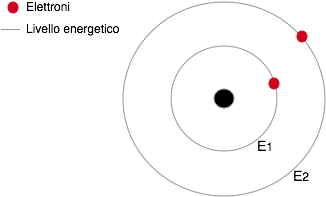
\includegraphics[scale=0.7]{cap1/atomico2liv}
    \caption{Sistema atomico composto da due livelli}
    \label{atomico2liv}
  \end{center}
\end{figure}

Quando la luce investe un materiale, si possono verificare due differenti tipi di transizione:
\begin{itemize}
	\item \emph{Assorbimento}: Quando il fascio di luce investe un materiale, parte dell'energia posseduta dal fascio viene ceduta. L'assorbimento consiste nel cedere, da parte del fotone, la propria energia al sistema atomico permettendo ad un singolo elettrone di passare da uno stato fondamentale $E_{1}$ ad uno stato eccitato $E_{2}$.
	\item \emph{Emissione}: Il sistema atomico cede energia al campo, in questo caso si possono avere due possibili scenari:
	\begin{itemize}
		\item \emph{Spontanea}: L'emissione spontanea si verifica quando un elettrone torna dal livello $E_{2}$ al livello $E_{1}$, provocando l'emissione di un fotone, senza nessun campo di radiazione incidente su di esso. Essa viene definita anche emissione incoerente: l'energia viene emessa con fase e direzione casuale.
		\item \emph{Stimolata}: L'emissione stimolata, invece, si ottiene quando un fotone incidente causa la discesa di un elettrone dal livello $E_{2}$ al livello $E_{1}$ ottenendo così due fotoni alla stessa frequenza. Quindi, in breve, un fotone colpisce l'atomo e due fotoni lo lasciano. Essa viene definita anche emissione coerente: l'energia viene emessa con la stessa fase, frequenza e direzione.
	\end{itemize} 
\end{itemize}
\begin{figure}[H]
  \begin{center}
    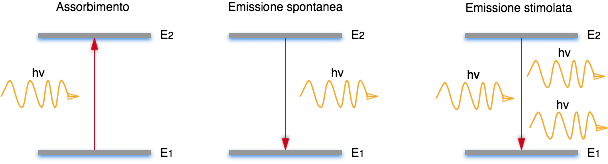
\includegraphics[scale=0.6]{cap1/funzatomoecc}
    \caption{Schema di funzionamento di un atomo eccitato: assorbimento, emissione spontanea ed emissione stimolata}
    \label{funzatomoecc}
  \end{center}
\end{figure}
L'importanza dell'emissione stimolata sta nel fatto che essendo prodotti due fotoni iso-frequenziali, di fatto avviene un'amplificazione ottica, la quale consente il funzionamento del sistema laser.

Per comprendere i meccanismi che regolano lo scambio di energia tra la radiazione ed il sistema atomico, è necessario introdurre la statistica di Boltzmann~\cite{kasap2012optoelectronics}. Attraverso tale statistica \'e possibile definire la popolazione, in termini di densit\'a, di un livello energetico all'equilibrio termico mediante la seguente relazione:
\begin{equation}
  N=N_0e^{{-\frac{E}{kT}}}
\end{equation}
dove $N_0$ \'e la popolazione iniziale in un dato livello energetico e $k= 1.38 \cdot 10^{-23} J / K$ \'e la costante di Boltzmann. %% TODO controlla notazione
 
 Indicando, quindi, con $N_1$ e $N_2$ il numero di atomi per unit\'a di volume (popolazione atomica) per i rispettivi livelli $E_1$ e $E_2$, possiamo ricavare il rapporto tra il numero di atomi nello stato fondamentale e quello nello stato eccitato, all'equilibrio termodinamico alla temperatura $T$, tramite la seguente equazione:
\begin{equation}
	\frac{N_2}{N_1}=e^{-\frac{\Delta E}{kT}} 
	\label{rappboltz}
\end{equation}
dove $\Delta E = E_2 - E_1$.

La condizione necessaria per avere emissione stimolata \'e l'inversione di popolazione tra i due livelli energetici, ovvero, il numero di atomi presenti nel livello eccitato deve essere maggiore di quello fondamentale ($N_2 > N_1$).

In un sistema a due livelli questa condizione non \'e realizzabile poich\'e, come possiamo osservare dall'equazione \ref{rappboltz} a causa della presenza dell'esponenziale negativo, $N_1$ risulta sempre maggiore di $N_2$, ovvero gli atomi a energia minima sono maggiori rispetto a quelli eccitati. 
\'E evidente dunque che, per avere una maggior probabilit\'a di emissione rispetto all'assorbimento, sia necessaria un'inversione di popolazione, ovvero $N_2 > N_1$.

Per ottenere la condizione di inversione di popolazione \'e quindi necessario l'utilizzo di un sistema atomico con almeno tre livelli energetici.

\subsection{Inversione di popolazione}
\begin{figure}[H]
  \begin{center}
    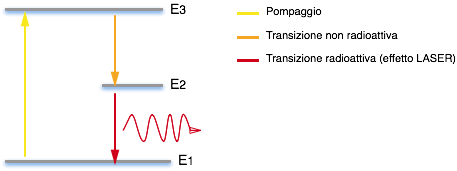
\includegraphics[scale=0.6]{cap1/sistema3liv}
    \caption{Sistema atomico a tre livelli energetici}
    \label{sistema3liv}
  \end{center}
\end{figure}
L'idea di base dell'inversione di popolazione consiste nello sfruttare i diversi tempi di vita medi dei differenti stati energetici.

Considerando un sistema ad esattamente tre livelli energetici ($E_1$, $E_2$ e $E_3$) schematizzato in Figura \ref{sistema3liv}, si sottopone il sistema atomico ad una radiazione luminosa di frequenza $\nu_{31}$, corrispondente al gap energetico $\Delta E_{31} = E_3-E_1$, in modo tale che gli elettroni dallo stato $E_1$ si eccitino raggiungendo lo stato instabile $E_3$. Questa prima fase è chiamata \emph{pompaggio}.

Successivamente si manifesta un decadimento dallo stato instabile $E_3$ allo stato $E_2$ in tempi molto rapidi e privi di emissione spontanea. Solitamente l'energia rilasciata viene trasferita sotto forma di moto vibrazionale al materiale circostante e non come fotone emesso.

Dal livello $E_2$ si verifica l'emissione laser alla frequenza $\nu_{21}$ e la conseguente regressione dal livello $E_2$ al livello $E_1$. La condizione necessaria, sui tempi di vita medi, per il funzionamento del laser è $\tau_{32} \ll \tau_{21}$, ovvero che il decadimento da $E_3$ a $E_2$ sia pi\'u rapido di quello da $E_2$ a $E_1$. Tale condizione permette di avere inversione di popolazione, ovvero $N_2 > N_1$, cos\'i da poter innescare l'amplificazione ottica e, quindi, l'effetto laser alla frequenza $\nu_{21}$.

Questo metodo \'e inefficiente perch\'e richiede un pompaggio elevato: \'e necessario fornire un numero elevato di elettroni al livello $E_3$ in modo tale che possa donarli al livello $E_2$ permettendo cos\'i l'inversione di popolazione.

Un struttura pi\'u efficiente \'e quella a quattro livelli schematizzata in Figura \ref{sistema4liv}. In questa disposizione, il pompaggio degli elettroni avviene da $E_1$ a $E_4$ a cui segue una transizione rapida e senza radiazione verso $E_3$ che consente di popolare il livello energetico. A questo punto avviene la transizione lenta e l'emissione tramite azione laser. Infine avviene una rapida transizione da $E_2$ allo stato fondamentale $E_1$.

\begin{figure}[H]
	\begin{center}
		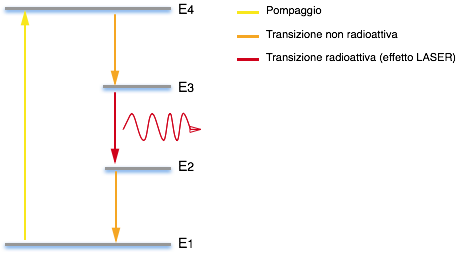
\includegraphics[scale=0.6]{cap1/sistema4liv}
		\caption{Sistema atomico a quattro livelli energetici}
		\label{sistema4liv}
	\end{center}
\end{figure}

A differenza della struttura a tre livelli, questa ha il vantaggio di avere il livello $E_3$ popolato mentre il livello $E_2$ vuoto ($N_2=0$), in quanto gli elettroni decadono rapidamente dallo stato $E_2$ allo stato $E_1$, aiutando a conservare l'inversione di popolazione $N_3 \gg N_2$. 
				
Oltre al meccanismo appena descritto, altre caratteristiche risultano cruciali nel funzionamento del laser: la \textit{cavit\'a ottica} e il \textit{materiale attivo}.

\subsection{Cavit\'a ottica e materiale attivo}
Nel paragrafo precedente abbiamo visto come realizzare un materiale amplificatore, che sfrutta l'inversione di popolazione nei livelli energetici. Per generare il fascio laser \'e necessario, per\'o, inserire il materiale attivo all'interno di una cavit\'a ottica.
Una semplice cavit\'a ottica può essere rappresentata dalla cavit\'a a specchi piani e paralleli, nota anche come cavit\'a di Fabry-Perot, mostrata in Figura \ref{cavitaottica}. 
\begin{figure}[H]
	\begin{center}
		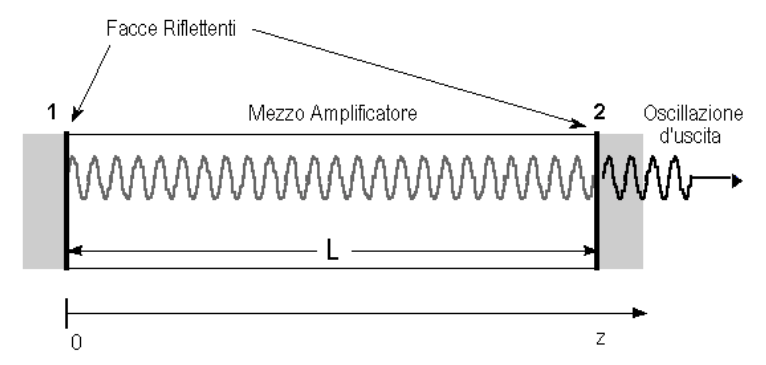
\includegraphics[scale=0.4]{cap1/cavitaottica}
		\caption{Cavit\'a di Fabry-Perot}
		\label{cavitaottica}
	\end{center}
\end{figure}
\begin{figure}[H]
  \begin{center}
    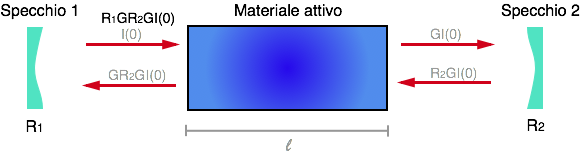
\includegraphics[scale=0.6]{cap1/roundtrip}
    \caption{Schema del Roundtrip ottico nella cavit\'a ottica}
    \label{roundtrip}
  \end{center}
\end{figure}
Il fascio di luce viaggia avanti-indietro riflettendosi negli specchi e amplificandosi nel passaggio all'interno del materiale attivo. Il fascio laser in uscita si ottiene rendendo uno dei due specchi della cavit\'a ottica parzialmente trasparente, in modo tale che parte della radiazione esca dalla cavit\'a.

Per definire il guadagno ottico del materiale attivo \'e necessario introdurre per\'o alcuni concetti preliminari. Indicando con $I$ l'intensità luminosa, definiamo l'intensità della luce all'interno della cavit\'a ottica con la seguente relazione:
\begin{equation}
I(l)=I(0)e^{\sigma(N_2-N_1)l}
\end{equation}
dove $\sigma$ \'e la la \textit{cross section} di emissione e $l$ \'e la lunghezza della cavit\'a ottica.

\begin{figure}[H]
  \begin{center}
    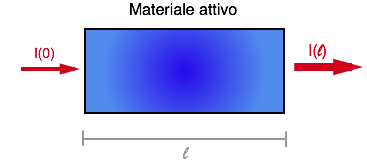
\includegraphics[scale=0.6]{cap1/propagazione}
    \caption{Propagazione della radiazione all'interno della cavità laser}
    \label{propagazione}
  \end{center}
\end{figure}
Possiamo definire il guadagno ottico del mezzo attivo come:
\begin{equation}
  G=\frac{I(l)}{I(0)}=e^{\sigma(N_2-N_1)l}
\end{equation}
sulla quale graveranno le limitazioni dovute alle perdite del materiale e alla perdita utile di potenza dovuta al laser uscente.

La cavità ottica e il mezzo attivo formano quindi un oscillatore ottico, ossia un amplificatore che viene retro-azionato positivamente attraverso specchi riflettenti posti ai lati del materiale attivo. Quindi, per avere un'azione laser è necessario raggiungere una situazione in cui il guadagno di amplificazione sia tale da compensare tutte le perdite presenti. 

Considerando come perdite solamente la riflettività parziale degli specchi $R_1$ e $R_2$, l'oscillazione ottica si innesca quando il guadagno del materiale attivo supera le perdite della cavità in un giro completo, o \textit{round trip}:
\begin{equation}
  G^2=\frac{1}{R_1R_2}
\end{equation}
Quest'ultimo è chiamato guadagno critico o inversione critica.

\section{Laser a semiconduttore}
Un dispositivo laser a semiconduttore utilizza una giunzione \textit{p-n} come materiale attivo all'interno della cavità ottica. Il pompaggio avviene tramite la ricombinazione di elettroni e lacune, che produce fotoni ad una lunghezza d'onda dipendente dal \textit{gap} tra i livelli energetici del dispositivo: la frequenza della radiazione emessa è legata quindi al tipo di materiali impiegati~\cite{sveltolaser}.

In commercio esistono diverse tipologie di laser a semiconduttore. Esse differiscono sulla base di due aspetti fondamentali: il tipo di cavità ottica impiegata e la forma degli specchi semi-riflettenti necessari a realizzare la retroazione ottica. 

Sulla base di queste due caratteristiche si possono individuare tre categorie principali di laser:
\begin{enumerate}
	\item Laser Fabry-Perot
	\item Laser DFB
	\item Laser VCSEL
\end{enumerate}

\subsection{Laser Fabry-Perot}
\begin{figure}[H]
  \begin{center}
    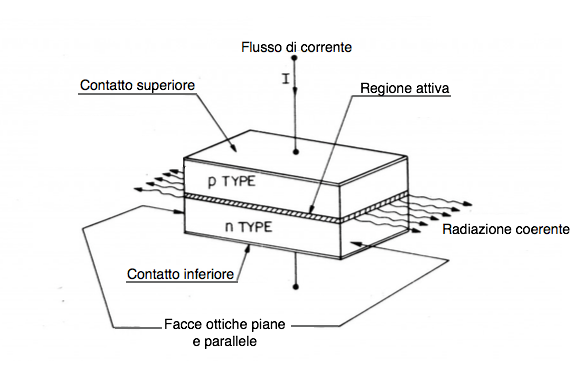
\includegraphics[scale=0.5]{cap1/fabryperot}
    \caption{Laser Fabry-Perot}
    \label{fabryperot}
  \end{center}
\end{figure}
I laser Fabry-Perot hanno la classica configurazione con cavità orizzontale a specchi piani, come mostrato in Figura \ref{fabryperot}.

Il principio di funzionamento é analogo a quello di un oscillatore ottico, descritto per esteso nel paragrafo precedente.

In particolare, la luce presente in cavità stimola alcuni atomi, già eccitati dalla corrente di pompa, ad emettere un fotone isofrequenziale con stessa fase di quello incidente.  
Gli specchi agli estremi della cavità rendono possibile la retroazione positiva, infatti fanno in modo che si possano instaurare alcuni modi di oscillazione stabili, o talvolta solo uno. 

Questo può rappresentare uno svantaggio in applicazioni come l'interferometria.

\subsection{Laser DFB}
\begin{figure}[H]
	\begin{center}
		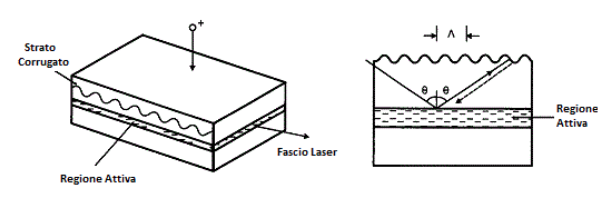
\includegraphics[scale=0.5]{cap1/dfb}
		\caption{Laser DFB}
		\label{dfb}
	\end{center}
\end{figure}
DFB è l'acronimo di \emph{Distributed Feedback Laser}. Il principio di funzionamento è simile a quello dei laser Fabry-Perot, ma con la importante differenza che non sono presenti due specchi separati a formare la cavità ottica ma è inserito uno strato corrugato adiacente allo strato attivo.

Questo strato aggiuntivo è fabbricato in maniera tale da riflettere solo una banda stretta di lunghezze d'onda, così da garantire un singolo modo longitudinale. 

Per questa caratteristica i laser DFB, sono più stabili dei Fabry-Perot, e più adatti ad applicazioni connesse alle fibre ottiche.

\subsection{Laser VCSEL}
\begin{figure}[H]
  \begin{center}
    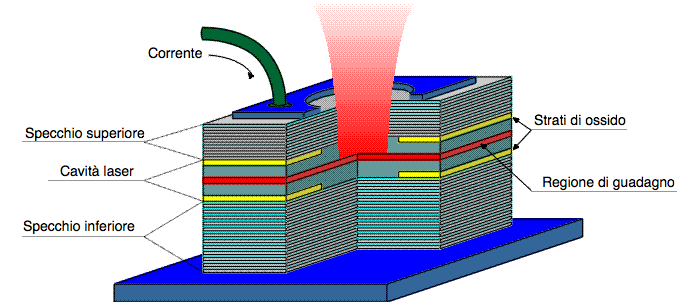
\includegraphics[scale=0.45]{cap1/vcsel}
    \caption{Laser VCSEL}
    \label{vcsel}
  \end{center}
\end{figure}
VCSEL è l'acronimo di \emph{Vertical Cavity Surface-Emitting Laser}. Questi dispositivi, a differenza delle precedenti due categorie, presentano una cavità ottica verticale. 

La cavità ottica ha una lunghezza molto inferiore alle dimensioni laterali del dispositivo, ciò implica che la luce del fascio laser viene emessa dalla superficie piuttosto che dai bordi laterali. 

Poiché la cavità risulta essere più ristretta rispetto alle altre tipologie, a parità di guadagno $G$ occorre aumentare la riflettività degli specchi per ottenere un guadagno d'anello maggiore di uno. A sfavore vi è una limitazione in potenza di emissione dovuta agli specchi altamente riflettenti.

\section{Classi di sicurezza dei laser}
Durante lo sviluppo di un sistema che include l'utilizzo di sorgenti laser è di fondamentale importanza garantire lo svolgimento del lavoro in sicurezza. Infatti, avendo a che fare con sorgenti laser, è importante conoscere i danni che esse possono provocare a cose e/o persone. In particolare, nei casi più gravi, le sorgenti laser possono procurare danni alla retina dell'occhio e ustioni alla pelle. 

Per poter scegliere in modo appropriato il laser da impiegare nel dispositivo è indispensabile conoscere le norme legislative che ne regolano l'utilizzo~\cite{ans}. A livello europeo vige la normativa \emph{IEC/EN 60825-1} che fissa una classificazione dei fasci laser in funzione della lunghezza d'onda e della potenza ottica emessa. 

La suddetta normativa classifica la pericolosità di una sorgente laser suddividendola in 4 classi:
\begin{itemize}
	\item \emph{Classe 1}: Questa classe include le sorgenti laser che non arrecano danni a cose e/o persone
	\item \emph{Classe 2}: Questa classe comprende i laser che emettono nell'intervallo di lunghezza d'onda compreso tra $400nm$ e $700nm$. Possono provocare danni alla retina dell'occhio in caso di osservazione prolungata.
	\item \emph{Classe 3}: Questa classe comprende due sotto-classi.
		\begin{itemize}
		\item \emph{Classe 3A}: Questa classe include tutte le sorgenti laser che risultano sicure per una visione naturale e non mediante strumenti ottici (es. microscopi)
		\item \emph{Classe 3B}: Questa classe include tutte le sorgenti laser che risultano pericolose per una visione naturale. \'E necessario utilizzare protezioni per gli occhi e disporre delle segnalazioni di avvertimento nella zona in cui si utilizza il laser. 
		\end{itemize}
	\item \emph{Classe 4}: Questa classe include le sorgenti laser più pericolose. Possono causare lesioni alla pelle e costituiscono pericolo d'incendio. 
\end{itemize}
\begin{figure}[H] 
  \begin{center}
    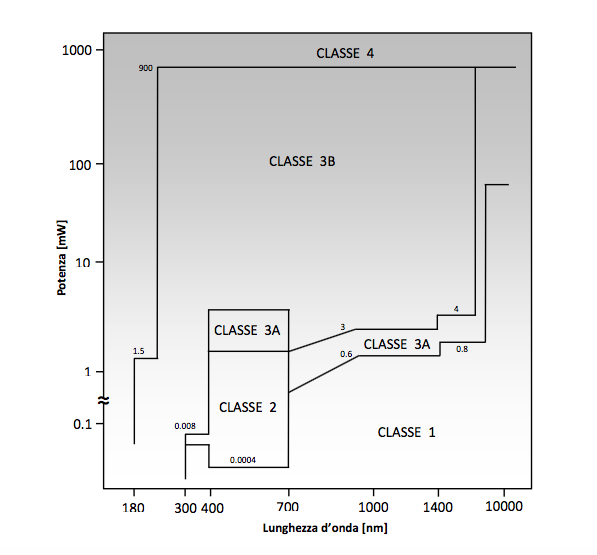
\includegraphics[scale=0.5]{cap1/classisicurezza}
    \caption{Classi di sicurezza dei laser}
    \label{classisicurezza}
  \end{center}
\end{figure}
La classificazione appena descritta è rappresentata in Figura \ref{classisicurezza}, insieme alle lunghezza d'onda corrispondenti a ciascuna classe.

\section{Telemetri ottici}
La telemetria è un insieme di metodi di osservazione aventi lo scopo di fornire la misura della distanza di un oggetto dall'osservatore.

Lo strumento che effettua la misura è chiamato telemetro: esso rileva la distanza assoluta tra lo strumento stesso e un oggetto remoto, chiamato bersaglio. In commercio esistono diverse tipologie di telemetri che si basano sull'impiego di sorgenti laser.

Le tipologie più diffuse sono tre: 
\begin{enumerate}
	\item A triangolazione
	\item A tempo di volo
	\item A onda continua
\end{enumerate}

\subsection{Telemetri a triangolazione}
\begin{figure}[H]
  \begin{center}
    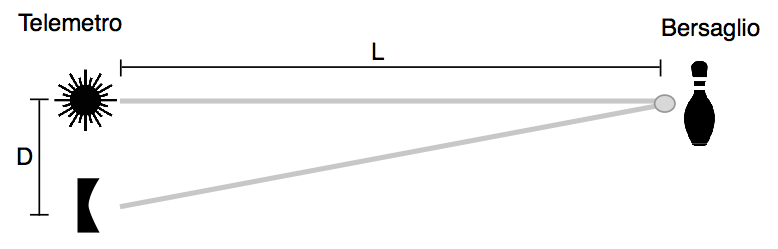
\includegraphics[scale=0.5]{cap1/triangolazione}
    \caption{Schema di funzionamento di un telemetro a triangolazione}
    \label{triangolazione}
  \end{center}
\end{figure}
I telemetri a triangolazione utilizzano una sorgente laser e un'ottica di ricezione posti perpendicolarmente ad una distanza $D$ tra loro. Inoltre, la sorgente laser è posizionata ad una distanza $L$ dal bersaglio. Si dice, quindi, che il bersaglio è "triangolato" da due punti a distanza $D$ su una stessa linea di base. Lo schema è mostrato in Figura \ref{triangolazione}.

Questo tipo di telemetro si basa sul principio della triangolazione, quindi valuta la distanza del bersaglio, conoscendo l'angolo $\alpha$ con cui il fascio laser viene riflesso sull'ottica di ricezione. 

Tramite questo angolo, infatti, è possibile ricavare la seguente relazione:
\begin{equation}
	\frac{D}{L}=\tan\alpha\approx\alpha
\end{equation}
Questa approssimazione è valida solo se $\alpha \ll 1$. 

L'angolo $\alpha$ si trova valutando la posizione in cui il fascio colpisce il fotorivelatore, secondo la relazione: 
\begin{equation}
  \alpha=\frac{x}{f_{rec}}
\end{equation}
dove $x$ è la distanza del punto di incidenza sul fotorivelatore dall'asse ottico della lente di ricezione, mentre $f_{rec}$ è la lunghezza focale dell'ottica di ricezione.

La misura della distanza si ricava facilmente dalle precedenti relazioni:
\begin{equation}
  L=\frac{D}{x}f_{rec}
\end{equation}
Differenziando quest'ultima equazione si trova l'errore di misura assoluto $\Delta L$ dovuto al minimo spostamento misurabile $\Delta x$ sul rivelatore: 
\begin{equation}
	 \Delta L=-\frac{D}{x^2}f_{rec}\Delta x
\end{equation}
Ricavando quindi un errore di misura relativo pari a:
\begin{equation}
\frac{\Delta L}{L}=-\frac{\Delta x}{x}=-\frac{\Delta\alpha}{\alpha}
\end{equation}
Il principale svantaggio di questa tecnica è che, con l'aumentare della distanza $L$, l'angolo $\alpha$ diminuisce, e ciò comporta l'aumento dell'incertezza relativa $-\frac{\Delta\alpha}{\alpha}$.
 
Per tale motivo, questa tipologia di telemetro è utilizzata per la misura di brevi distanze ($0.1\div 10 m$) .

\subsection{Telemetri a tempo di volo}
\begin{figure}[H]
	\begin{center}
		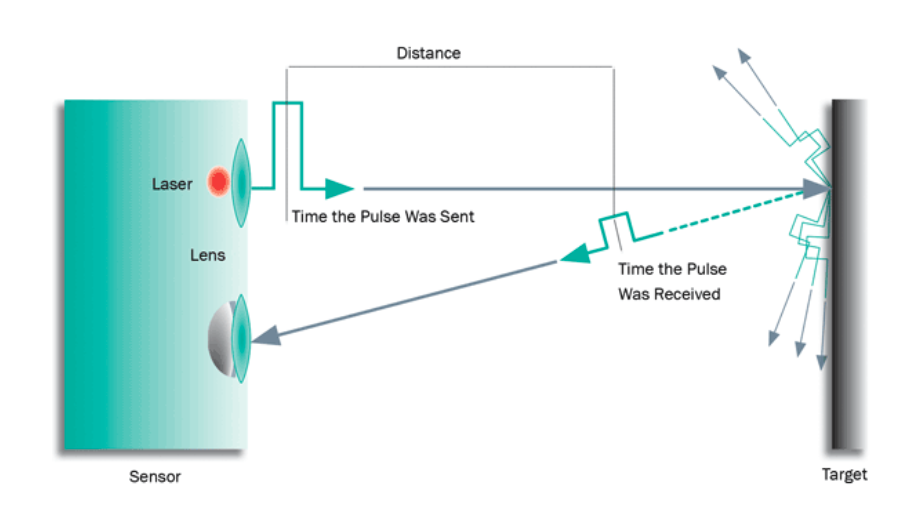
\includegraphics[scale=0.4]{cap1/tempodivolo}
		\caption{Schema di funzionamento di un telemetro a tempo di volo}
		\label{tempodivolo}
	\end{center}
\end{figure}
I telemetri a tempo di volo utilizzano un laser impulsato. Essi emettono potenza solo per un brevissimo istante di tempo $\tau$.

Con un bersaglio posto a distanza $L$ dalla sorgente laser, il fascio laser percorre un cammino pari a $2L$ (Andata e Ritorno) in un tempo $T$ viaggiando a velocità della luce $c\approx3\cdot10^8\frac{m}{s}$, ricavando così la seguente relazione:
\begin{equation}
  L=\frac{c}{2}T
\end{equation}
Differenziando la precedente equazione si ottiene:
\begin{equation}
  \Delta L=\frac{c}{2}\Delta T
\end{equation}

Da cui si ricava la relazione:

\begin{equation}
  \frac{\Delta L}{L}=\frac{\Delta T}{T}
\end{equation}
Si può osservare come la misura $\Delta L$ dipenda unicamente dal $\Delta T$ che si riesce a risolvere. In pratica, la misura viene effettuata utilizzando un contatore che conta quanti tempi di clock $\Delta T$ sono intercorsi tra l'istante di partenza del raggio laser e il momento in cui ritorna all'ottica di rivelazione.

Il vincolo di questi telemetri è che la durata dell'impulso $\tau$ deve soddisfare la condizione $\tau \ll \Delta T$. Per tale motivo sono utilizzati per misure di distanze medio-lunghe (fino a $10 Km$). 

\subsection{Telemetri a onda continua}
\begin{figure}[H]
  \begin{center}
    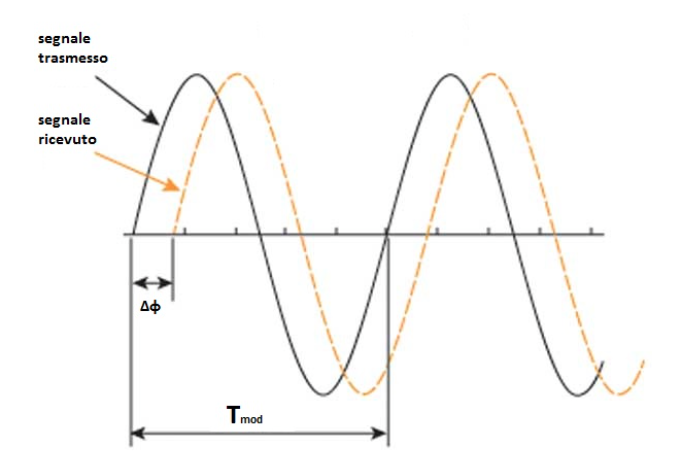
\includegraphics[scale=0.4]{cap1/ondacontinua}
    \caption{Potenza trasmessa e potenza riflessa in un telemetro a onda continua}
    \label{ondacontinua}
  \end{center}
\end{figure}
I telemetri a onda continua hanno un funzionamento analogo ai telemetri a tempo di volo, ma a differenza di questi ultimi, la potenza ottica viene modulata sinusoidalmente a frequenza $f_{mod}$ ottenendo il segnale in Figura \ref{ondacontinua}.

La potenza trasmessa dal laser vale quindi:
\begin{equation}
	 P(t)=P_0[1+msin(2\pi f_{mod}t)]
\end{equation} 
Nella pratica, la misura non viene effettuata con un contatore elettronico, come per i telemetri a tempo di volo, ma avviene mediante la rilevazione del ritardo di fase $\Delta\phi$ tra il segnale ricevuto $P_r$ e il segnale trasmesso $P_t$.

Considerando la relazione:
\begin{equation}
  \frac{\Delta\phi}{2\pi}=\frac{\Delta t}{T_{mod}}
\end{equation}
dove $\Delta t=\frac{2L}{c}$ e $T_{mod}=\frac{1}{f_{mod}}$, si ottiene così la misura di distanza assoluta:
\begin{equation}
  L=\frac{c}{2}\frac{1}{2\pi f_{mod}}\Delta\phi=\frac{\Delta\phi}{S}
\end{equation}
Dall'ultima equazione si può notare come la sensibilità $S=2 \frac{2\pi f_{mod}}{c}$ della misura migliori all'aumentare della frequenza di modulazione. Tuttavia un aumento eccessivo della frequenza di modulazione comporta una riduzione della massima distanza rilevabile. 

Questo tipo di telemetro si utilizza per misure comprese tra $1 \div 1000m$, con risoluzioni dell'ordine del millimetro. 

\section{Una tecnica alternativa per la misura}
Come già discusso nell'Introduzione, lo scopo di questo lavoro di Tesi è realizzare il prototipo di un misuratore di distanza assoluta che sia a basso costo e con ingombro limitato per poter essere più maneggevole nella misura di medio-brevi distanze.

Da quanto esposto nel precedente paragrafo, emerge che i telemetri descritti non sono in grado di raggiungere tali obiettivi. Infatti tali strumenti sono adatti per la misura di distanze dell'ordine della decina di metri. Per quanto riguarda i telemetri a triangolazione, invece, esistono in commercio strumenti in grado di misurare distanze brevi con buona sensibilità. Tuttavia questi dispositivi, oltre ad avere un costo elevato, necessitano di un'ottica specifica per la ricezione della radiazione riflessa e di un bersaglio cooperativo.

Da queste osservazioni si conclude che, per raggiungere l'obiettivo preposto, è necessario utilizzare una tecnica di misura che si differenzia da quelle comuni, ovvero l'\textbf{interferometria a retroiniezione}. Questa tecnica verrà ampiamente discussa nel Capitolo \ref{capitolo2}.











 







